\section{Component architecture}
A component architecture diagram is useful to illustrate how a system is connected.
A component architecture is a system structure composed of interconnected components, where components are a collection of program parts that constitute a whole \cite{OOAD}.
\autoref{fig:architecture-diagram} shows the component architecture.

\begin{figure}[]
    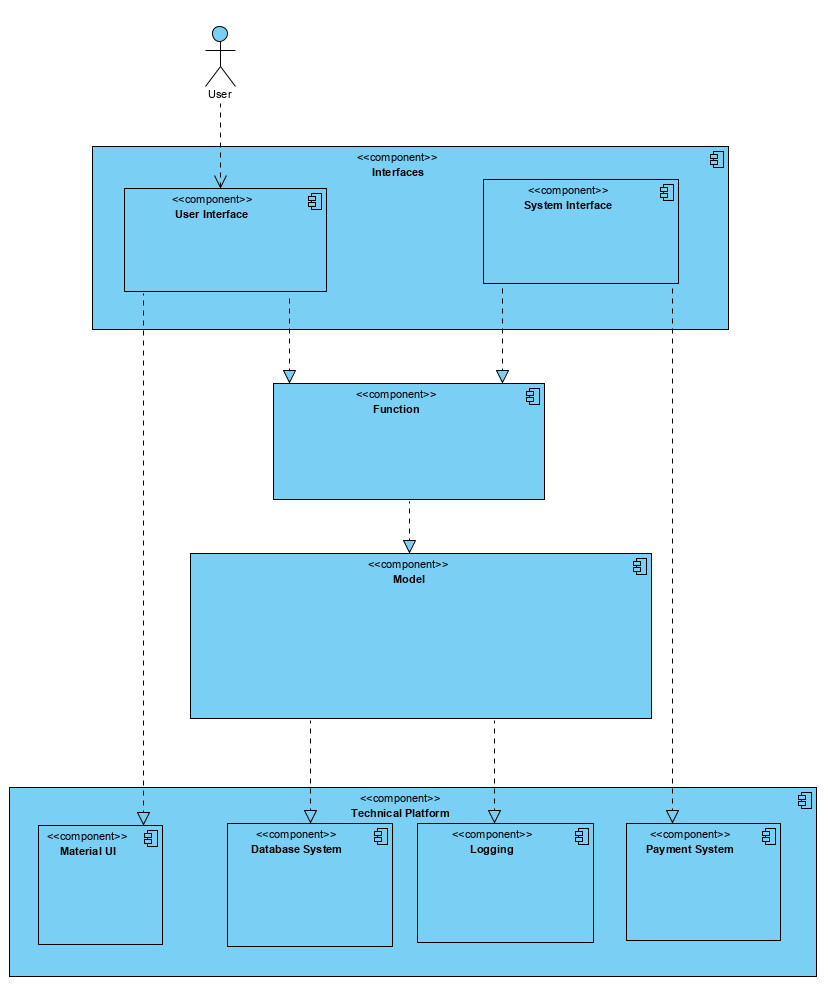
\includegraphics[width=\linewidth]{/architecture.PNG}
    \caption{The component architecture of the system}
    \label{fig:architecture-diagram}
\end{figure}

\subsection{Interfaces}
The top component layer of the system is the \textit{Interfaces} layer.
This layer defines the components that interact with other entities, such as users or other systems, which is how the layer is split.
The user of the system interacts with the user interface.
The user interface has an interface to the \textit{Technical Platform} component layer, more specifically the \textit{Material UI} component.
Material UI is the framework used to create the user interface, which is why they interface.
The user interface also interfaces with the \textit{Function} component, in order to facilitate interaction with the system when used by a user. 
The \textit{System Interface} component interfaces with the \textit{Payment System} from the \textit{Technical Platform}, since a payment system should be used to facilitate transactions.
It also interfaces with the \textit{Function} component, to facilitate interaction with the system.

\subsection{Function and Model components}
The \textit{Function} and \textit{Model} components define the core functionalities of the system.
The function component takes the necessary information from the system and user interfaces, and ensures it can be used by the model.
For example, a user inputs certain information when registering. 
The function component then takes this information, ensures it has the proper format and passes it to the model component.
The model component takes information from the function component, and interfaces with the \textit{Technical Platform}.
From the \textit{Technical Platform} layer it interfaces with the \textit{Database System} and the \textit{Logging} component.
The model's content is received and stored in the \textit{Database System}.
Whenever certain actions are performed through user actions, the \textit{Logging} component takes the relevant model content and logs it.
\\\\
Now that the architecture has been defined and prototypes created, we will discuss how, and with which frameworks we will be creating the front end.

